In simulated and real experiments, we find that our method gives more accurate predictions than alternatives and is substantially faster than existing methods that share information across time intervals. Each of our experiments explores a different application with a different natural reference family.

\textbf{Baselines.} We compare to three other methods, all described in \cref{sec:intro}. (1) A vanilla multimarginal SB (\textit{\vanilla{}}) with a Brownian motion reference. See \cref{sec:vanilla-app} for implementation details.
(2) The Deep Momentum multimarginal Schr\"odinger bridge (\textit{\dmsbname{}}) \citep{chen2024deep}. We use the authors' code at \href{https://github.com/TianrongChen/DMSB.}{\nolinkurl{https://github.com/TianrongChen/DMSB}}; see \cref{sec:dmsb-app} for details. (3) \textit{TrajectoryNet} \citep{tong2020trajectorynet}. We use the code at \href{https://github.com/KrishnaswamyLab/TrajectoryNet}{\nolinkurl{https://github.com/KrishnaswamyLab/TrajectoryNet}}; see \cref{app:trajnetdetails}. In all SB methods, we set the volatility $\volatility$ to 0.1, as suggested by \citet{Vargas2021}. See \cref{app:train-hyperparams-ref} for implementation details of our method. 

\textbf{Measuring accuracy.} In each experiment, we start with a collection of data at an odd total number of time points. We train each method using data from odd-indexed times (including the first and last time points); we use even-indexed times as held-out validation data. At a high level, we measure accuracy by how well the empirical distribution of a method's simulated trajectories corresponds to held-out data at each validation time point. We evaluate the performance both visually and via numerical summaries of error. 

Since all methods estimate drift, it should be possible to simulate trajectories from all training particles for all methods. However, the \dmsbname{} code provides trajectories originating only from the first-time-point particles, and the TrajectoryNet code provides trajectories originating only from the final-time-point particles. Therefore, to provide a more direct comparison of trajectory quality, we plot only the subset of trajectories provided by our method and \vanilla{} that arise from the first-time-point particles.

We report numerical summaries for our method both for these restricted trajectories and also for trajectories using all particles. In practice, we recommend practitioners use our full method with all particles; we consider restricted trajectories only for comparison to existing, restricted code.
While we focus on the Earth Mover's Distance (EMD) in the main text, we also compute the Maximum Mean Discrepancy (MMD) in \cref{app:further-experiments}. We discuss these choices in \cref{app:metrics}.

In each table entry, we report the mean and standard deviation of each result across 10 random seeds.
We report results on the restricted set of trajectories in the first rows of each table, and results over all possible trajectories in the final rows.
We highlight (in green) the best restricted result (across methods), and any other (restricted) method whose one-standard-deviation confidence interval
overlaps the mean of the best (restricted) method. We highlight (in light blue) any all-trajectory method that beats the best restricted result or any all-trajectory method whose one-standard-deviation confidence interval
overlaps the mean of the best restricted method. We provide more details in \cref{app:tiebreaking}. Our conclusions generally agree across all metrics.

\begin{figure*}[!ht]
    \centering
    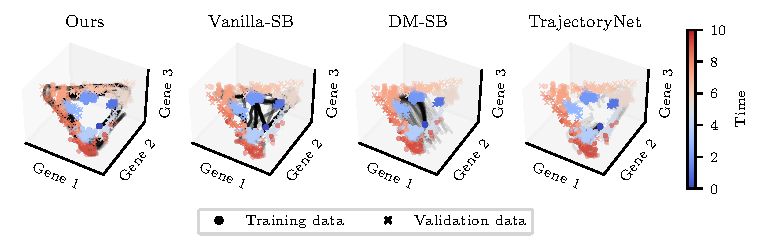
\includegraphics[width = .95\textwidth]{./Figs/repr50_trajectories.pdf}
    \caption{\label{fig:repr-main} 
    Comparison on the repressilator synthetic data (\cref{sec:represmain}) with 6 training times, 5 validation times, and 50 observations per time. Each plot shows 50 simulated trajectories, originating from particles at one time end point (three left plots: first time; right plot: final time).}
\end{figure*}

\textbf{Measuring runtime.} We describe our run time comparisons in detail, and provide full running time results, in \cref{app:timing-table}. We emphasize that implementation details affect runtime, which can be hard to interpret for iterative SB methods without clear stopping criteria. For instance, our method may slow down with more iterations and samples due to our piece-wise SB solver choice, but could also be accelerated with faster piece-wise SB solvers. Similarly, other methods may benefit from fewer iterations or improved SDE solvers. Therefore, these reported runtimes should be interpreted in the context of each experiment's specific setup.


\subsection{Lotka-Volterra} 
\label{sec:LVmain}
We generate synthetic data from a stochastic Lotka-Volterra predator-prey model; we use the same parametric dynamical system as the reference family in our method. We take 5 training and 4 validation time points, with 50 observations per time point. See \cref{app:lv-app} for more details.

\textbf{Accuracy.} In \cref{fig:LV-main}, we see that, since \vanilla{} learns drift by interpolating between each pair of time points, it misses the curvature of the dynamics. TrajectoryNet misses the curvature of the initial time points. While both \dmsbname{} and our method capture the overall curvature, the enforced smoothness of \dmsbname{}'s trajectories lead to substantial mass away from the validation data (as in the lower left corner) and worse EMD performance; see \cref{tab:LV50_EMD_appendix}.


\textbf{Runtime.} Across the 10 seeds, we find the following runtimes in hours, reported as mean $\pm$ one standard deviation: \dmsbname{} 7.62$\pm$3.18, TrajectoryNet 10.96$\pm$0.81, ours 0.61$\pm$0.12, and \vanilla{} 0.06$\pm$0.01. Of the methods incorporating information across multiple time intervals, our method is (on average across runs) the fastest.
%12 times faster than \dmsbname{} and 18 times faster than TrajectoryNet; 
\vanilla{} is the fastest due to its relative simplicity. Since \vanilla{} is a subroutine in our method, we expect our method to be about $K$ times as expensive. TrajectoryNet is built on constrained continuous normalizing flows, which are known to be computationally intensive \citep{grathwohl2018ffjord}.
We conjecture that \dmsbname{} faces computational challenges due to learning dynamics in a larger space (velocity and location vs.\ just location), with no direct observations in the velocity part of the space. In the context of generative modeling using diffusion, \citet{dockhorn2021score} also augment their model with particle velocities and face increased training time.

\subsection{Repressilator} 
\label{sec:represmain}
We generate synthetic data based on a model that captures the circadian rhythm in cyanobacteria \citep{nakajima2005reconstitution}. Three coupled SDEs model mRNA levels of three genes that cyclically suppress each other's synthesis. We use the same parametric dynamics as the reference family in our method. We take 6 training and 5 validation times, with 50 observations per time. See \cref{app:repr-app} for more details.

\textbf{Accuracy.} In \cref{fig:repr-main}, we see that \vanilla{}, \dmsbname{}, and TrajectoryNet all fail to capture the cyclic nature of these dynamics. But our method accurately captures the curvature. The EMD summaries agree that our method outperforms the alternatives; see \cref{tab:repres50_EMD_appendix}.

\textbf{Runtime.} Across the 10 seeds, we find the following runtimes in hours (mean $\pm$ one standard deviation): \dmsbname{} 15.63$\pm$0.12, TrajectoryNet 9.86$\pm$0.43, ours 2.43$\pm$0.60, and \vanilla{} 0.23$\pm$0.05. Our method is (on average across runs) faster than all the baselines sharing information across intervals.
%over 6 times as fast as \dmsbname{} and over 4 times as fast as TrajectoryNet; 
Again, our method offers substantial accuracy gains at a lower computational cost.

\begin{figure*}[!ht]
    \centering
    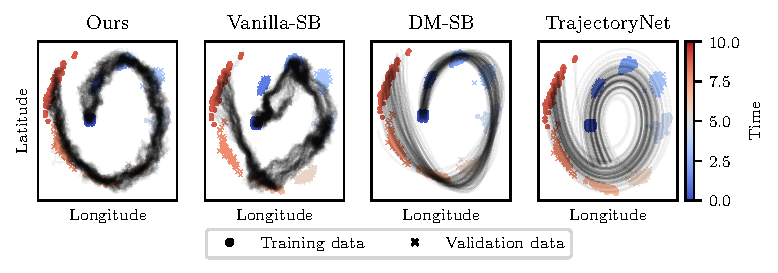
\includegraphics[width =.97\textwidth]{Figs/GoMsmall_trajectories.pdf}
    \caption{    Comparison on the Gulf of Mexico data (\cref{sec:gommain}) with 5 training times, 4 validation times, and approximately 111 observations per time. Each plot shows approximately 111 simulated trajectories, originating from particles at one time end point (three left plots: first time; right plot: final time). 
    }
    \label{fig:GoMsmall-main}
\end{figure*}

\subsection{Ocean currents in the Gulf of Mexico}
\label{sec:gommain}
In our remaining two analyses, our reference family is mis-specified; that is, since we use real data, the reference family cannot exactly match the data-generating process. 
We first use real ocean-current data from the Gulf of Mexico: we use high-resolution (1 km) bathymetry data from a HYbrid Coordinate Ocean Model (HYCOM) reanalysis\footnote{Dataset available at \url{https://www.hycom.org/data/gomb0pt01/gom-reanalysis}.} to obtain a velocity field around what appears to be a vortex feature. We simulate particles (representing buoys or ocean debris) that evolve according to this field. We observe a total of 1000 particles across 5 training and 4 validation times. In our method, we use a reference parametric family representing a vortex with unknown center,
direction, and shape. See \cref{app:GoM-app-reference} for full details.  

\textbf{Accuracy.} In \cref{fig:GoMsmall-main}, \vanilla{} produces polygon-like ``kinks" --- i.e., sharp turns in trajectories --- at training time points. These kinks represent a failure to capture a smooth vortex motion aligned with fluid dynamics principles. These artifacts arise because \vanilla{}'s drift is learned strictly from pairwise time intervals, instead of incorporating information from the entire time horizon. \dmsbname{} and TrajectoryNet generate smooth trajectories that are notably far from the data at the final validation time point. Our method's trajectories track the validation data closely. Our EMD results in \cref{tab:GoMsmall_EMD_appendix} reflect that both our method and \dmsbname{} are close to the data at the first 3 validation time points. But \dmsbname{} is about twice as far (in EMD) relative to our method (or to either method at other validation points) at the final validation point. We provide results for an additional experiment on particles farther from the center of the vortex in \cref{app:GoM-app-results}. 


\textbf{Runtime.} Across the 10 seeds, we find the following runtimes in hours (mean $\pm$ one standard deviation): \dmsbname{} 15.44$\pm$0.02, TrajectoryNet 7.44$\pm$0.25, ours 4.67$\pm$0.66, and \vanilla{} 0.43$\pm$0.01. Of the methods sharing information across multiple time intervals, our method is (on average across runs) the fastest.
%over 3.3 times as fast as \dmsbname{} and over 1.6 times as fast as TrajectoryNet; 

\subsection{Single-cell sequencing} 
\label{sec:scrnamain}
We next consider two single-cell sequencing datasets. We follow  \citet{tong2020trajectorynet,chen2024deep} in analyzing data from \citet{moon2019visualizing} on embryoid body (EB) cells. We analyze an additional dataset from \citet{chu2016single} on human embryonic stem cells (hESC). Both datasets promise insight into the dynamic process of stem cell differentiation. 
We use the same pre-processing pipeline of \citet{tong2020trajectorynet} for the EB data, and we apply this pipeline to the hESC data.
The EB data has 3 training and 2 validation time points. We subsample it to have 300 cells at each time.
The hESC dataset initially has 6 time points. We remove the final time point so that we start and end with training times. The resulting training times have 92, 66, 138 cells, and the validation times have 102, 172 cells, respectively.

For the reference family input to our method, we use a gradient field family, following \citet{wang2011quantifying, weinreb2018fundamental, lavenant2024toward}. This family is motivated by Waddington's famous analogy between cellular differentiation and a marble rolling down a potential surface \citep{waddington2014strategy}. 
To parameterize the gradient field in our experiment, we use a multilayer perceptron (MLP), an architecture commonly used for gradient field representations \citep[e.g.,][]{greydanus2019hamiltonian,lin2023computing}. Our MLP consists of three hidden layers with sizes 128, 64, and 64, interconnected by ReLU activation functions. We choose this specific configuration, including sizes and training hyperparameters, by doing a grid search detailed in \cref{app:eb_implementation}. 

\textbf{Accuracy.} We see from \cref{tab:EB_EMD} that, when comparing the quality of only those trajectories generated from a single end point in time, \dmsbname{} outperforms the alternatives, including our method. However, when allowed to generate trajectories from all particles, \vanilla{} and our method outperform the single-time trajectory options (as expected) and perform comparably to each other. Indeed, when we look at the data itself (\cref{fig:eb-app} for EB, \cref{fig:hesc-app} for hESC), it appears that there is not much pattern in the data on the time scale at which the data is sampled; the EB data in particular appears to move in a single direction. In neither the EB nor hESC case do we see a clear and meaningful visual pattern that any method picks up. We emphasize that the number of training time points is only three, so there is not much pattern that could be picked up. With all of these considerations in mind, we conjecture that \dmsbname{} and TrajectoryNet would perform about as well as the \vanilla{} method or our method in these two cases if they were used to generate trajectories from all training particles; we are not able to confirm with the existing code.

\begin{table*}[!ht]
    \centering
    \begin{tabular}{lcccc}
    \hline
       & \multicolumn{2}{c}{EB} & \multicolumn{2}{c}{hESC} \\
        Method & EMD $t_2$ & EMD $t_4$ & EMD $t_2$ & EMD $t_4$ \\
    \hline
        \vanillaonetime & 1.49 $\pm$ 0.063 & 1.55 $\pm$ 0.034 & 1.47 $\pm$ 0.088 & 1.97 $\pm$ 0.169\\
         \dmsb & \cellcolor{green!25}\textbf{1.13 $\pm$ 0.082} & \cellcolor{green!25}\textbf{1.45 $\pm$ 0.16} & \cellcolor{green!25}\textbf{1.10 $\pm$ 0.066} & 1.51 $\pm$ 0.11\\
         \trajnet & 2.03 $\pm$ 0.04 & 1.93 $\pm$ 0.08 & 1.30 $\pm$ 0.04 & 1.93 $\pm$ 0.05 \\
         \oursonetime & 1.27 $\pm$ 0.028 & 1.57 $\pm$ 0.048 & \cellcolor{green!25}\textbf{1.08 $\pm$ 0.12} & \cellcolor{green!25}\textbf{1.33 $\pm$ 0.084} \\
    \hline
        \vanillaalltime & \cellcolor{blue!10}\textbf{1.12 $\pm$ 0.031} & \cellcolor{blue!10}\textbf{1.12 $\pm$ 0.023} & \cellcolor{blue!10}\textbf{0.72 $\pm$ 0.017} & \cellcolor{blue!10}\textbf{1.27 $\pm$ 0.043} \\
        \oursalltime & \cellcolor{blue!10}\textbf{0.96 $\pm$ 0.019} & \cellcolor{blue!10}\textbf{1.19 $\pm$ 0.017} & \cellcolor{blue!10}\textbf{0.71 $\pm$ 0.031} & \cellcolor{blue!10}\textbf{1.25 $\pm$ 0.076} \\
    \hline
    \end{tabular}
    \caption{Earth mover's distance (mean $\pm$ standard deviation) at 2 validation times for the EB and hESC data. The first four rows use only trajectories generated from one time endpoint. The final two rows use all trajectories. }
    \label{tab:EB_EMD}
\end{table*}

\textbf{Runtime.} First consider EB. Across the 10 seeds, we find the following runtimes in hours (mean $\pm$ one standard deviation): \dmsbname{} 15.54$\pm$0.41, TrajectoryNet 10.19$\pm$0.37, ours 0.38$\pm$0.05, and \vanilla{} 0.03, with a standard deviation less than 0.01. Of the methods sharing information across multiple time intervals, our method is (on average across runs) the fastest.
%over 41 times as fast as \dmsbname{} and about 27 times as fast as TrajectoryNet; 
Next consider hESC. We find the following runtimes in hours: \dmsbname{} 15.40$\pm$0.08, TrajectoryNet 8.00$\pm$0.49, ours 0.56$\pm$0.04, and \vanilla{} 0.05, with a standard deviation less than 0.01. Also for this experiment, our method is (on average across runs) the fastest.
%over 27 times as fast as \dmsbname{} and about 14 times as fast as TrajectoryNet; 




